\section{Consuntivo di periodo}
Il team \textit{Club Swendwitch} di seguito espone i dati ottenuti dall'esperienza concreta di sviluppo del progetto.
Vengono evidenziate inoltre le differenze rispetto a quanto esposto nel preventivo analizzato nella sezione precedente. 

\subsection{Analisi}
\newcolumntype{P}[1]{>{\centering\arraybackslash}p{#1}}
{\renewcommand{\arraystretch}{1.8}
    \begin{center}
        \begin{tabular}{P{0.25\linewidth}P{0.15\linewidth}P{0.20\linewidth}}
            \rowcolor[RGB]{33, 73, 50}
            \textcolor{white}{\textbf{Ruolo}} & \textcolor{white}{\textbf{Ore}} & \textcolor{white}{\textbf{Costo}}\\
            \rowcolor[RGB]{216, 235, 171}
            Responsabile & 25 \textcolor{red}{(+5)} & 750\euro \space \textcolor{red}{(+150\euro)}\\
                
            \rowcolor[RGB]{233, 245, 206}
            Amministratore & 20 \textcolor{red}{(+4)}& 400\euro \space \textcolor{red}{(+80\euro)}\\
    
            \rowcolor[RGB]{216, 235, 171}
            Analista & 45 \textcolor{red}{(+5)} & 1125\euro \space \textcolor{red}{(+125\euro)}\\
    
            \rowcolor[RGB]{233, 245, 206}
            Progettista & - & -\\
    
            \rowcolor[RGB]{216, 235, 171}
            Programmatore & - & -\\
    
            \rowcolor[RGB]{233, 245, 206}
            Verificatore & 45 \textcolor{red}{(+5)} & 675\euro \space \textcolor{red}{(+75\euro)}\\
    
            \arrayrulecolor{white}\hline\hline
    
            \rowcolor[RGB]{216, 235, 171}
            Totale Preventivo & 116 & 2520\euro\\

            \rowcolor[RGB]{233, 245, 206}
            \textbf{Totale Consuntivo} & 135 \textcolor{red}{(+19)} & 2950\euro \space \textcolor{red}{(+430\euro)}\\
        \end{tabular}
        \captionof{table}{Consuntivo orario - Analisi}
    \end{center}
}
\begin{figure}[h!]
	\centering
	\includegraphics[scale=0.37]{../../assets/Diagrammi_Excel/torta_ore_Analisi.png}
	\caption{Ripartizione percentuale oraria dei ruoli - Analisi}
\end{figure}

\subsubsection{Considerazioni}
In questa prima fase il gruppo \textit{Club Swendwitch} ha visto un incremento delle ore rispetto a quanto riportato nel preventivo. Questo aumento è sicuramente dovuto all'inesperienza generale del gruppo, il quale ha trovato difficoltà nell'analisi del capitolato C5 - Login Warrior e nella conseguente organizzazione dei compiti.\\
\'E sicuramente stato un fattore rilevante il fatto che il preventivo redatto sia stato particolarmente ottimista e non abbia tenuto conto di eventuali problematiche organizzative che si sono presentate, come mostrato nella sezione \hyperref[sec:AttualizzazioneRischi]{\textit{Attualizzazione dei rischi}}

\subsection{Technology baseline e codifica del PoC}
{\renewcommand{\arraystretch}{2.0}
    \begin{center}
        \begin{tabular}{P{0.25\linewidth}P{0.15\linewidth}P{0.20\linewidth}}
            \rowcolor[RGB]{33, 73, 50}
            \textcolor{white}{\textbf{Ruolo}} & \textcolor{white}{\textbf{Ore}} & \textcolor{white}{\textbf{Costo}}\\
            \rowcolor[RGB]{216, 235, 171}
            Responsabile & 16 \textcolor{red}{(+2)} & 480\euro \space \textcolor{red}{(+60\euro)}\\
                
            \rowcolor[RGB]{233, 245, 206}
            Amministratore & 6 \textcolor{blue}{(-2)} & 120\euro \space \textcolor{blue}{(-40\euro)} \\
    
            \rowcolor[RGB]{216, 235, 171}
            Analista & 12 \textcolor{red}{(+5)} & 300\euro \space \textcolor{red}{(+125\euro)}\\
    
            \rowcolor[RGB]{233, 245, 206}
            Progettista & 25 \textcolor{red}{(+5)} & 625\euro \space \textcolor{red}{(+125\euro)}\\
    
            \rowcolor[RGB]{216, 235, 171}
            Programmatore & 30 \textcolor{red}{(+5)} & 450\euro \space \textcolor{red}{(+75\euro)}\\
    
            \rowcolor[RGB]{233, 245, 206}
            Verificatore & 20 \textcolor{red}{(+5)} & 300\euro \space \textcolor{red}{(+75\euro)}\\
    
            \arrayrulecolor{white}\hline\hline
    
            \rowcolor[RGB]{216, 235, 171}
            Totale Preventivo & 89 & 1855\euro\\
    
            \rowcolor[RGB]{233, 245, 206}
            \textbf{Totale Consuntivo} & 109 \textcolor{red}{(+20)} & 2275\euro \space \textcolor{red}{(+420\euro)}\\
        \end{tabular}
        \captionof{table}{Consuntivo orario - Technology baseline}
    \end{center}    
}
\begin{figure}[h!]
	\centering
	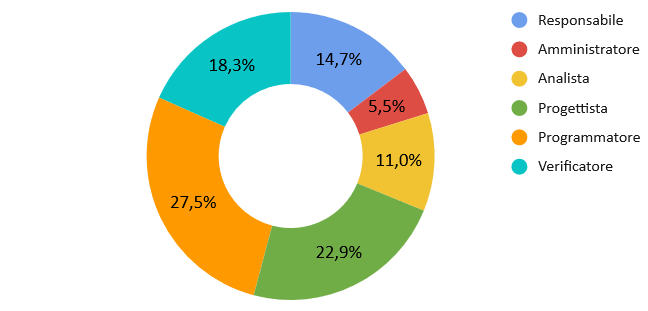
\includegraphics[scale=0.37]{../../assets/Diagrammi_Excel/torta_ore_TB.png}
	\caption{Ripartizione percentuale oraria dei ruoli - Technology baseline}
\end{figure}

\subsection{Considerazioni}
In questa fase il gruppo \textit{Club Swendwitch} ha riscontrato un incremento delle ore su quasi tutti i ruoli ad eccezione del ruolo di amministratore. Le motivazioni che hanno portato all'aumentare delle ore necessarie sono sicuramente: l'inesperienza del gruppo con le tecnologie utilizzate (come \textit{React}$^{G}$ e \textit{D3.js}$^{G}$), 
l'attuale situazione pandemica e l'accavallarsi degli esami universitari, come mostrato nella sezione \hyperref[sec:AttualizzazioneRischi]{\textit{Attualizzazione dei rischi}}.\\
L'unico ruolo che ha migliorato le aspettative è stato l'amministratore: gli strumenti scelti per l'organizzazione delle tasks hanno funzionato egregiamente, semplificando molto il lavoro e portando ad una riduzione sul consuntivo di fase di circa due ore.

\subsection{Riepilogo consuntivo}
{\renewcommand{\arraystretch}{2.0}        
        \begin{tabular}{P{0.25\linewidth}P{0.07\linewidth}P{0.07\linewidth}P{0.07\linewidth}P{0.08\linewidth}P{0.08\linewidth}P{0.08\linewidth}P{0.08\linewidth}}
            \rowcolor[RGB]{33, 73, 50}
            \textcolor{white}{\textbf{Nominativo}} & \textcolor{white}{\textbf{RE}} &
            \textcolor{white}{\textbf{AM}} & \textcolor{white}{\textbf{AN}} &
            \textcolor{white}{\textbf{PT}} & \textcolor{white}{\textbf{PG}} &
            \textcolor{white}{\textbf{VE}} & \textcolor{white}{\textbf{Tot.}}\\
        
            \rowcolor[RGB]{216, 235, 171}
            Barilla Gianmarco & 
            0 \par \textcolor{blue}{(-2)} & 
            2 \par \textcolor{blue}{(-1)} & 
            7 \par \textcolor{blue}{(-1)} & 
            3 \par \textcolor{red}{(+1)} & 
            0 & 
            14 \par \textcolor{red}{(+3)} &
            26 \\
            
            \rowcolor[RGB]{233, 245, 206}
            Beni Valentina & 
            13 \par \textcolor{red}{(+4)} & 
            6 \par \textcolor{red}{(+1)} & 
            16 \par \textcolor{red}{(+5)} & 
            5 \par \textcolor{red}{(+2)} &
            0 \par \textcolor{blue}{(-5)}&
            20 \par \textcolor{red}{(+10)}& 
            60 \par \textcolor{red}{(+18)}\\

            \rowcolor[RGB]{216, 235, 171}
            Bustaffa Marco & 
            15 \par \textcolor{red}{(+7)}& 
            6 \par \textcolor{red}{(+1)} &      
            15 \par \textcolor{red}{(+5)} & 
            3 \par \textcolor{red}{(+1)} &
            0 \par \textcolor{blue}{(-5)} &
            11 \par \textcolor{red}{(+1)}&
            50 \par \textcolor{red}{(+10)}\\

            \rowcolor[RGB]{233, 245, 206}
            Canel Alessandro & 
            0 \par \textcolor{blue}{(-2)} & 
            3 & 
            6 & 
            3 \par \textcolor{red}{(+1)} & 
            0 & 
            11 & 
            23 \par \textcolor{blue}{(-1)}\\

            \rowcolor[RGB]{216, 235, 171}
            Ferrarini Alessio & 
            4 \par \textcolor{blue}{(-2)}& 
            2 \par \textcolor{blue}{(-1)} &   
            5 & 
            8 \par \textcolor{red}{(+1)} &
            30 \par \textcolor{red}{(+20)}&
            0 \par \textcolor{blue}{(-5)}& 
            49 \par \textcolor{red}{(+13)}\\

            \rowcolor[RGB]{233, 245, 206}
            Pozzebon Samuele & 
            9 \par \textcolor{red}{(+2)}& 
            7 \par \textcolor{red}{(+2)}&      
            8 \par \textcolor{red}{(+1)} & 
            3 \par \textcolor{blue}{(-2)}& 
            0 \par \textcolor{blue}{(-5)}&
            9 \par \textcolor{red}{(+1)} & 
            36 \par \textcolor{blue}{(-1)}\\

            \arrayrulecolor{white}\hline\hline

            \rowcolor[RGB]{216, 235, 171}
            \textbf{Totale ore ruolo} & 
            41 \par \textcolor{red}{(+7)} & 
            26 \par \textcolor{red}{(+2)} & 
            57 \par \textcolor{red}{(+10)} & 
            23 \par \textcolor{red}{(+3)} &
            30 \par \textcolor{red}{(+5)}& 
            65 \par \textcolor{red}{(+10)}& 
            244 \par \textcolor{red}{(+39)}\\

            \rowcolor[RGB]{233, 245, 206}
            \textbf{Totale costi ruolo} & 
            1230\euro \par \textcolor{red}{(+210)}& 
            520\euro \par \textcolor{red}{(+40)}& 
            1425\euro \par \textcolor{red}{(+250)}& 
            625\euro \par \textcolor{red}{(+125)}& 
            450\euro \par \textcolor{red}{(+75)}& 
            975\euro \par \textcolor{red}{(+150)}& 
            5225\euro \par \textcolor{red}{(+850)}
        \end{tabular}
        \captionof{table}{Riepilogo finale del consuntivo}
}

\begin{figure}[h!]
	\centering
	\begin{minipage}[c]{0.42\textwidth}
    	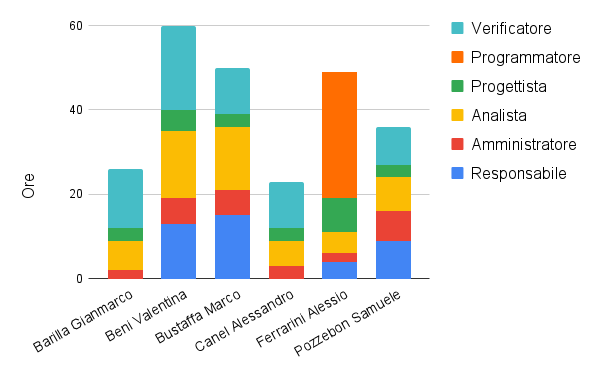
\includegraphics[scale=0.38]{../../assets/Diagrammi_Excel/consuntivo_tot_rtb.png}
		\caption{Riepilogo consuntivo - \\ruoli per persona}
	\end{minipage}
\hfill
	\begin{minipage}[c]{0.47\textwidth}
		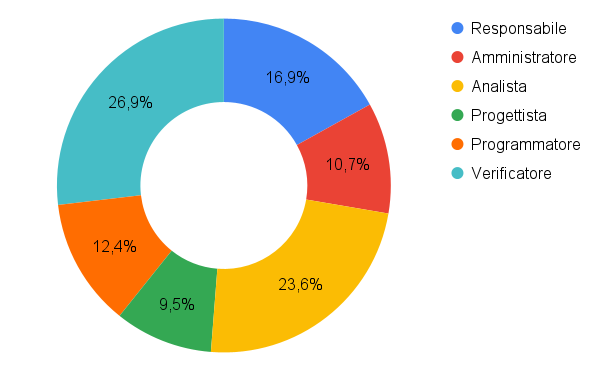
\includegraphics[scale=0.38]{../../assets/Diagrammi_Excel/torta_tot_rtb.png}
		\caption{Riepilogo consuntivo - \\ripartizione percentuale oraria}
	\end{minipage}
\end{figure}


% TO DO: METTERE LE CAPTIONS ALLE TABELLE
